\documentclass[xcolor={table}]{beamer}
\usepackage{fleqn}
\usepackage{graphicx}
\usepackage{coordsys} %for \numbline commander

%Setup appearance:
\usetheme{Darmstadt}
\usefonttheme[onlylarge]{structurebold}
\setbeamerfont*{frametitle}{size=\normalsize,series=\bfseries}
\setbeamertemplate{navigation symbols}{}
\setbeamertemplate{bibliography item}{[\theenumiv]}

% Standard packages
\usepackage[english]{babel}
\usepackage[latin1]{inputenc}
\usepackage{times}
\usepackage[T1]{fontenc}
\usepackage{multirow}
\usepackage{subfigure}
\usepackage{pbox}
\usepackage{arydshln}
\usepackage{pifont}
\usepackage{cancel}
\usepackage{rotating} % for sideways headings

% Source Code packages
\usepackage{algorithm2e}
\usepackage{algorithmic}

\DeclareSymbolFont{extraup}{U}{zavm}{m}{n}
\DeclareMathSymbol{\varclub}{\mathalpha}{extraup}{84}
\DeclareMathSymbol{\varspade}{\mathalpha}{extraup}{85}
\DeclareMathSymbol{\varheart}{\mathalpha}{extraup}{86}
\DeclareMathSymbol{\vardiamond}{\mathalpha}{extraup}{87}

%%% This section command that adds a big page with section dividers
\usepackage{xifthen}% provides \isempty test
\newcommand{\SectionSlide}[2][]{
	\ifthenelse{\isempty{#1}}
		{\section{#2}\begin{frame} \begin{center}\begin{huge}#2\end{huge}\end{center}\end{frame}}
		{\section[#1]{#2}\begin{frame} \begin{center}\begin{huge}#2\end{huge}\end{center}\end{frame}}
}
%Extends the section slide to to include a shortened section title for the navigation bar as a second parameter
\newcommand{\SectionSlideShortHeader}[3][]{
	\ifthenelse{\isempty{#1}}
		{\section[#3]{#2}\begin{frame} \begin{center}\begin{huge}#2\end{huge}\end{center}\end{frame}}
		{\section[#1]{#2}\begin{frame} \begin{center}\begin{huge}#3\end{huge}\end{center}\end{frame}}
}

\newcommand{\refer}[1]{\footnote{#1}}
\newcommand{\GW}{\text{\textit{Guess-Who~}}}
\newcommand{\keyword}[1]{\alert{\textbf{#1}}\index{#1}}
\newcommand{\firstkeyword}[1]{\textbf{#1}\index{#1}}
\newcommand{\indexkeyword}[1]{\alert{\textbf{#1}\index{#1}}}
\newcommand{\featN}[1]{\textsc{#1}}
\newcommand{\featL}[1]{\textit{'#1'}}
 \newcommand{\ourRef}[1]{\ref{#1} $^{\text{\tiny[\pageref{#1}]}}$}
 \newcommand{\ourEqRef}[1]{\eqref{#1}$^{\text{\tiny[\pageref{#1}]}}$}
  
\DeclareMathOperator*{\argmax}{argmax}
\DeclareMathOperator*{\argmin}{argmin}



\title{Case Study - Customer Churn}
	\author{John D. Kelleher and Brian Mac Namee and Aoife D'Arcy}
	\institute{}
	\date{}

\begin{document}
\begin{frame}
	\titlepage
\end{frame}
\begin{frame}
	 \tableofcontents
\end{frame}

 \begin{frame} 
 \begin{itemize}
\item Acme Telephonica (AT) is a mobile phone operator that has customers across every state of the U.S.A. 
\item AT struggles with customer \keyword{churn prediction}---customers leaving AT for other mobile phone operators. 
\item In 2010 AT hired Ross, a predictive data analytics specialist, to take a new approach to reducing customer churn. 
\item This case study describes the work carried out by Ross when he took AT through the CRISP-DM process to develop a predictive data analytics  solution to this business problem. 
 \end{itemize}
 \end{frame} 
 
\SectionSlide{Business  Understanding}

 \begin{frame} 
 \begin{itemize}
\item AT did not approach Ross with a well-specified predictive analytics solution. Instead, the company approached him with a business problem---reducing customer churn. 
\item Ross's first goal was to convert this business problem into a concrete analytics solution. 
\item Before attempting this conversion, Ross had to fully understand the business objectives of AT. 
 \end{itemize}
 \end{frame} 
 
\SectionSlide{Data Understanding}


 \begin{frame} 
\begin{figure}[htb]
	\centering
	\includegraphics[width=0.9\textwidth]{./images/acmetelephone_mod.pdf}
	\caption{The set of domain concepts for the Acme Telephonica customer churn prediction problem.}
	\label{fig:ATChurnPredictionDataConcepts}
\end{figure}
\end{frame} 



 \begin{frame} [plain]
\label{tab:telcoAnalyticsBaseTable}
\centering
\begin{scriptsize}
\resizebox{\linewidth}{!}{\begin{tabular}{ p{3.5cm} p{8cm} }
\hline
Feature & Description\\
\hline
\featN{billAmountChangePct}	&		The percent by which the customer's bill has changed from last month to this month		\\
\featN{callMinutesChangePct}	&		The percent by which the call minutes used by the customer has changed from last month to this month		\\
\featN{avgBill}	&		The  average monthly bill amount		\\
\featN{avgRecurringCharge}	&		The average monthly recurring charge paid by the customer		\\
\featN{avgDroppedCalls}	&		The average number of customer calls dropped each month		\\
\featN{peakRatioChangePct}	&		The percent by which the customer's peak calls to off-peak calls ratio has changed from last month to this month		\\
\featN{avgReceivedMins}	&		The average number of calls received each month by the customer		\\
\featN{avgMins}	&		The average number of call minutes used by the customer each month		\\
\featN{avgOverBundleMins}	&		The average number of out-of-bundle minutes used by the customer each month		\\
\featN{avgRoamCalls}	&		The average number of roaming calls made by the customer each month		\\
\featN{peakOffPeakRatio}	&		The ratio between peak and off peak calls made by the customer this month	\\
\featN{newFrequentNumbers}	&		How many new numbers the customer is frequently calling this month?		\\
\hline
\end{tabular}}
\end{scriptsize}
\end{frame} 

 \begin{frame} [plain]
\label{tab:telcoAnalyticsBaseTable}
\centering
\begin{scriptsize}
\resizebox{\linewidth}{!}{\begin{tabular}{ p{3.5cm} p{8cm} }
\hline
Feature & Description\\
\hline
\featN{customerCareCalls}	&		The number of customer care calls made by the customer last month		\\
\featN{numRetentionCalls}	&		The number of times the customer has been called by the retention team		\\
\featN{numRetentionOffers}	&		The number of retention offers the customer has accepted		\\
\featN{age}	&		The customer's age		\\
\featN{creditRating}	&		The customer's credit rating		\\
\featN{income}	&		The customer's income level		\\
\featN{lifeTime}	&		The number of months the customer has been with AT		\\
\featN{occupation}	&		The customer's occupation		\\
\featN{regionType}	&		The type of region the customer lives in		\\
\featN{handsetPrice}	&		The price of the customer's current handset		\\
\featN{handsetAge}	&		The age of the customer's current handset		\\
\featN{numHandsets}	&		The number of handsets the customer has had in the past 3 years		\\
\featN{smartPhone}	&		Is the customer's current handset a smart phone?		\\
\featN{churn}	&		The target feature		\\
\hline
\end{tabular}}
\end{scriptsize}
\end{frame} 

\SectionSlide{Data Preparation}



 \begin{frame} [plain]
\centering
\begin{scriptsize}
\label{table:dataQualityReportATABTCont}\resizebox{\linewidth}{!}{\begin{tabular}{  l  c  r  c r  r r r r r r}
\hline
~	 & ~ & \% & ~ & ~	 & $1^{st}$	& ~ & ~ & $3^{rd}$  & ~  & Std.  \\
Feature	 & Count & Miss. & Card. & Min.	 & Qrt.	& Mean & Median & Qrt.  & Max.  & Dev.  \\
\hline
\featN{age}	&	10,000	&	11.47	&	40	&	0.00	&	0.00	&	30.32	&	34.00	&	48.00	&	98.00	&	22.16	\\
\featN{income}	&	10,000	&	0.00	&	10	&	0.00	&	0.00	&	4.30	&	5.00	&	7.00	&	9.00	&	3.14	\\
\featN{numHandsets}	&	10,000	&	0.00	&	19	&	1.00	&	1.00	&	1.81	&	1.00	&	2.00	&	21.00	&	1.35	\\
\featN{handsetAge}	&	10,000	&	0.00	&	1,923	&	52.00	&	590.00	&	905.52	&	887.50	&	1,198.00	&	2,679.00	&	453.75	\\
\featN{handsetPrice}	&	10,000	&	0.00	&	16	&	0.00	&	0.00	&	35.73	&	0.00	&	59.99	&	499.99	&	57.07	\\
\featN{avgBill}	&	10,000	&	0.00	&	5,588	&	0.00	&	33.33	&	58.93	&	49.21	&	71.76	&	584.23	&	43.89	\\
\featN{avgMins}	&	10,000	&	0.00	&	4,461	&	0.00	&	150.63	&	521.17	&	359.63	&	709.19	&	6,336.25	&	540.44	\\
\featN{avgrecurringCharge}	&	10,000	&	0.00	&	1,380	&	0.00	&	30.00	&	46.24	&	44.99	&	59.99	&	337.98	&	23.97	\\
\featN{avgOverBundleMins}	&	10,000	&	0.00	&	2,808	&	0.00	&	0.00	&	40.65	&	0.00	&	37.73	&	513.84	&	81.12	\\
\featN{avgRoamCalls}	&	10,000	&	0.00	&	850	&	0.00	&	0.00	&	1.19	&	0.00	&	0.26	&	177.99	&	6.05	\\
\featN{callMinutesChangePct}	&	10,000	&	0.00	&	10,000	&	-16.422	&	-1.49	&	0.76	&	0.50	&	2.74	&	19.28	&	3.86	\\
\featN{billAmountChangePct}	&	10,000	&	0.00	&	10,000	&	-31.67	&	-2.63	&	2.96	&	1.96	&	7.56	&	42.89	&	8.51	\\
\featN{avgReceivedMins}	&	10,000	&	0.00	&	7,103	&	0.00	&	7.69	&	115.27	&	52.54	&	154.38	&	2,006.29	&	169.98	\\
\featN{avgOutCalls}	&	10,000	&	0.00	&	524	&	0.00	&	3.00	&	25.29	&	13.33	&	33.33	&	610.33	&	35.66	\\
\featN{avgInCalls}	&	10,000	&	0.00	&	310	&	0.00	&	0.00	&	8.37	&	2.00	&	9.00	&	304.00	&	17.68	\\
\featN{peakOffPeakRatio}	&	10,000	&	0.00	&	8,307	&	0.00	&	0.78	&	2.22	&	1.40	&	2.50	&	160.00	&	3.88	\\
\featN{peakOffPeakRatioChangePct}	&	10,000	&	0.00	&	10,000	&	-41.32	&	-6.79	&	-0.05	&	0.01	&	6.50	&	37.78	&	9.97	\\
\featN{avgDroppedCalls}	&	10,000	&	0.00	&	1,479	&	0.00	&	0.00	&	0.50	&	0.00	&	0.00	&	9.89	&	1.41	\\
\featN{lifeTime}	&	10,000	&	0.00	&	56	&	6.00	&	11.00	&	18.84	&	17.00	&	24.00	&	61.00	&	9.61	\\
\featN{lastMonthCustomerCareCalls}	&	10,000	&	0.00	&	109	&	0.00	&	0.00	&	1.74	&	0.00	&	1.33	&	365.67	&	5.76	\\
\featN{numRetentionCalls}	&	10,000	&	0.00	&	5	&	0.00	&	0.00	&	0.05	&	0.00	&	0.00	&	4.00	&	0.23	\\
\featN{numRetentionOffersAccepted}	&	10,000	&	0.00	&	5	&	0.00	&	0.00	&	0.02	&	0.00	&	0.00	&	4.00	&	0.155	\\
\featN{newFrequentNumbers}	&	10,000	&	0.00	&	4	&	0.00	&	0.00	&	0.20	&	0.00	&	0.00	&	3.00	&	0.64	\\
\hline
\end{tabular}}
\end{scriptsize}
\end{frame} 

 \begin{frame} [plain]
\centering
\begin{scriptsize}
\label{table:dataQualityReportATABTCat}\resizebox{\linewidth}{!}{\begin{tabular}{  l  c r c c r r c r r}
\hline
~ & ~ & ~ & ~	 & ~	 & ~ & ~ & ~	& $2^{nd}$ & $2^{nd}$  \\
~ & ~ & \% & ~	 & ~	 & Mode & Mode & $2^{nd}$	& Mode & Mode  \\
Feature	& Count & Miss. & Card. & Mode	 & Freq. & \% & Mode	& Freq. & \%  \\
\hline
\featN{occupation}	&	10,000	&	74.00	&	8	&	professional	&	1,705	&	65.58	&	crafts	&	274	&	10.54	\\		
\featN{regionType}	&	10,000	&	47.80	&	8	&	suburb	&	3,085	&	59.05	&	town	&	1,483	&	28.39	\\		
\featN{marriageStatus}	&	10,000	&	0.00	&	3	&	unknown	&	3,920	&	39.20	&	yes	&	3,594	&	35.94	\\		
\featN{children}	&	10,000	&	0.00	&	2	&	FALSE	&	7,559	&	75.59	&	TRUE	&	2,441	&	24.41	\\		
\featN{smartPhone}	&	10,000	&	0.00	&	2	&	TRUE	&	9,015	&	90.15	&	FALSE	&	985	&	9.85	\\		
\featN{creditRating}	&	10,000	&	0.00	&	7	&	B	&	3,785	&	37.85	&	C	&	1,713	&	17.13	\\		
\featN{homeOwner}	&	10,000	&	0.00	&	2	&	FALSE	&	6,577	&	65.77	&	TRUE	&	3,423	&	34.23	\\		
\featN{creditCard}	&	10,000	&	0.00	&	6	&	TRUE	&	6,537	&	65.37	&	FALSE	&	3,146	&	31.46	\\		
\featN{churn}	&	10,000	&	0.00	&	2	&	FALSE	&	5,000	&	50.00	&	TRUE	&	5,000	&	50.00	\\		
\hline
\end{tabular}}
\end{scriptsize}
\end{frame} 



 \begin{frame} [plain]
 \begin{figure}[htb]
\centering
	\subfigure[\featN{income}]{\label{fig:acmeABTHistogramIncome}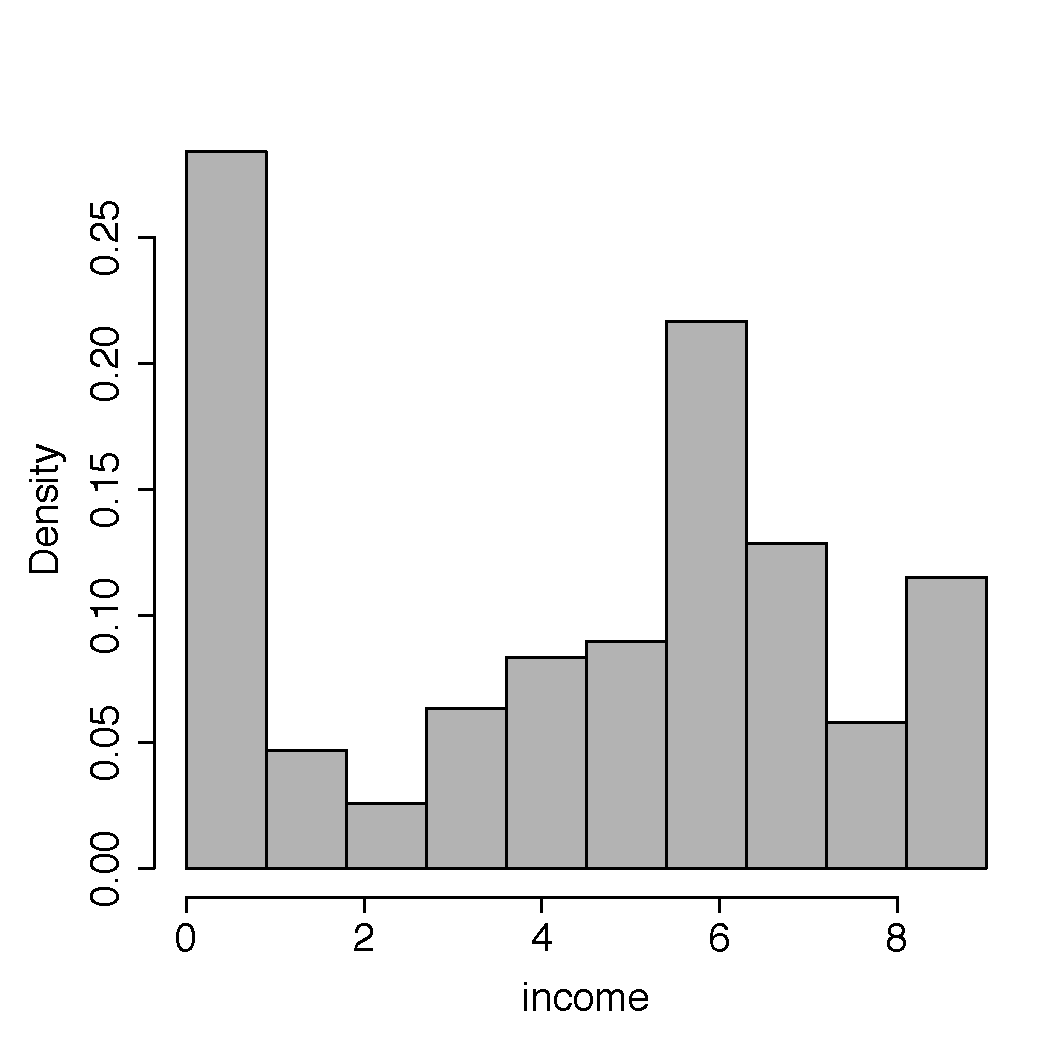
\includegraphics[width=0.24\linewidth]{./images/CaseStudy1_AcmeDQ_income_hist_All}}
	\subfigure[\featN{creditCard}]{\label{fig:acmeABTBarPlotCreditCard}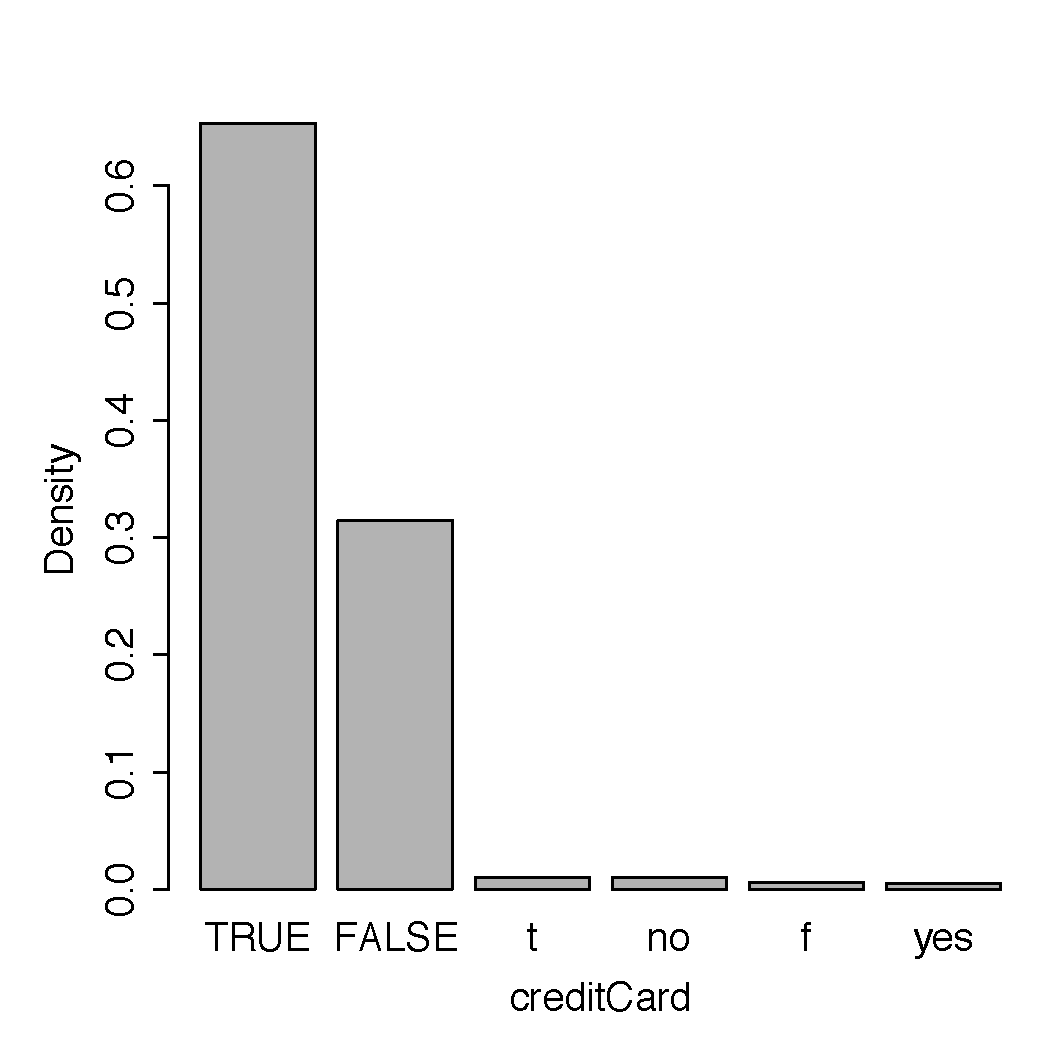
\includegraphics[width=0.24\linewidth]{./images/CaseStudy1_AcmeDQ_creditCard_bar_All.pdf}}
	\subfigure[\featN{regionType}]{\label{fig:acmeABTBarPlotRegionType}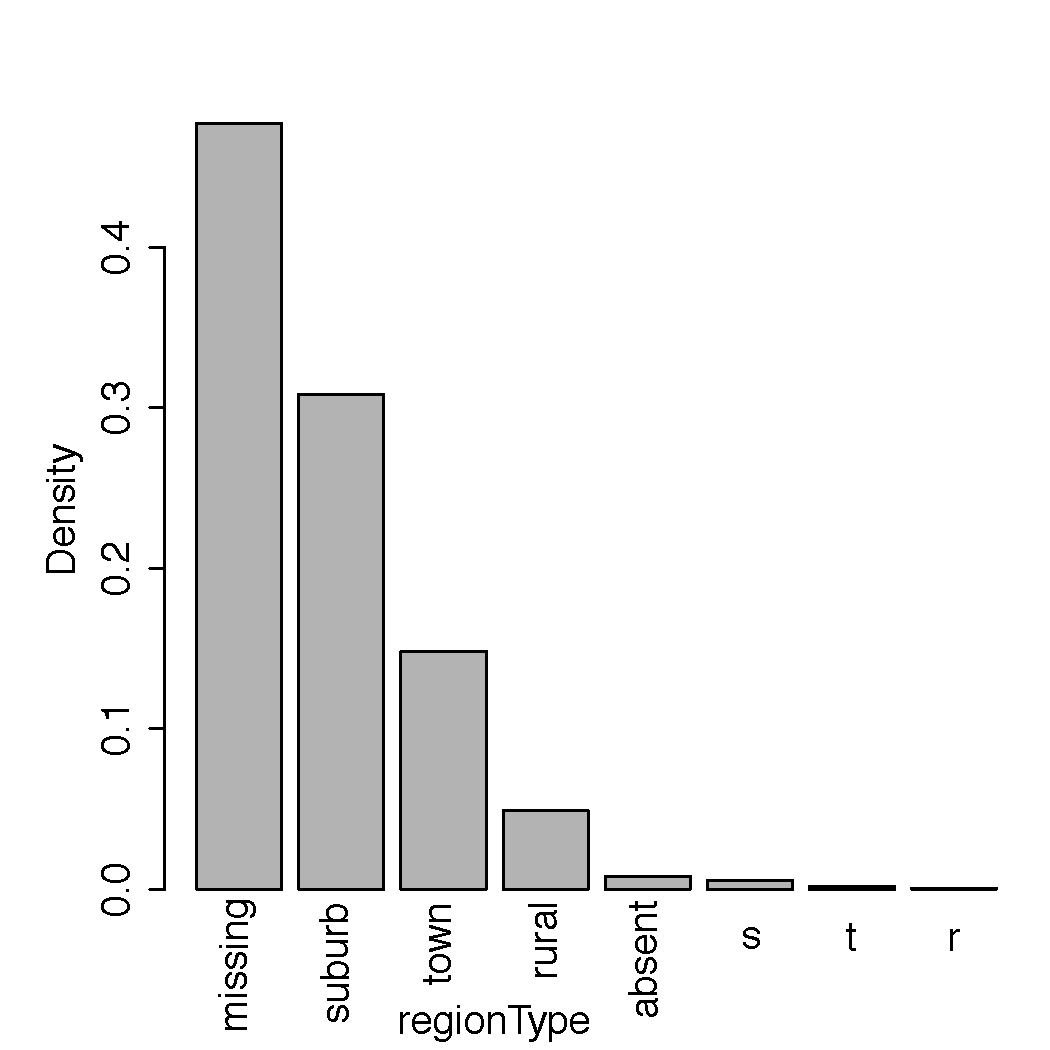
\includegraphics[width=0.24\linewidth]{./images/CaseStudy1_AcmeDQ_regionType_bar_All.pdf}}
	\subfigure[\featN{handsetPrice}]{\label{fig:acmeOutlierHistogram1}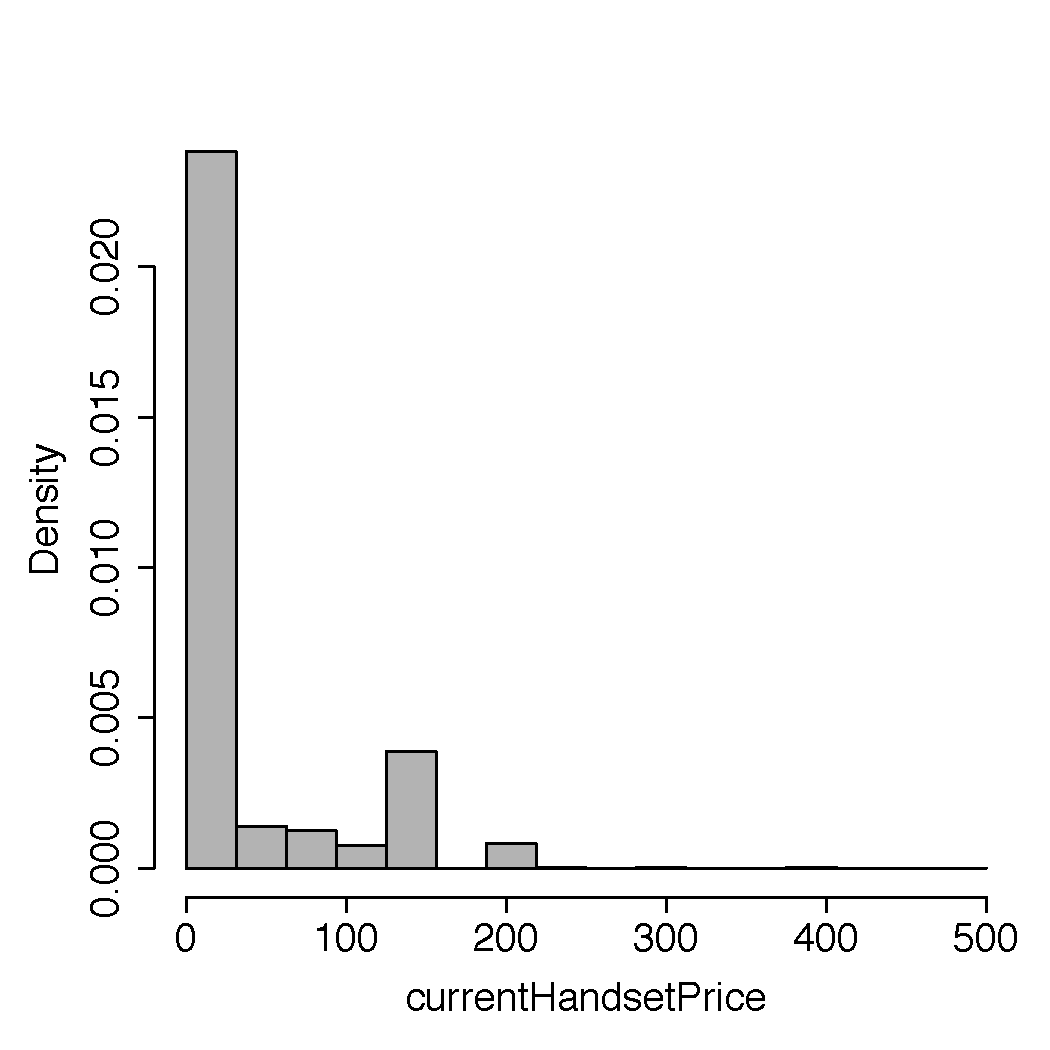
\includegraphics[width=0.24\linewidth]{./images/CaseStudy1_AcmeDQ_currentHandsetPrice_hist_All.pdf}}
	\subfigure[\featN{avgMins}]{\label{fig:acmeOutlierHistogram2}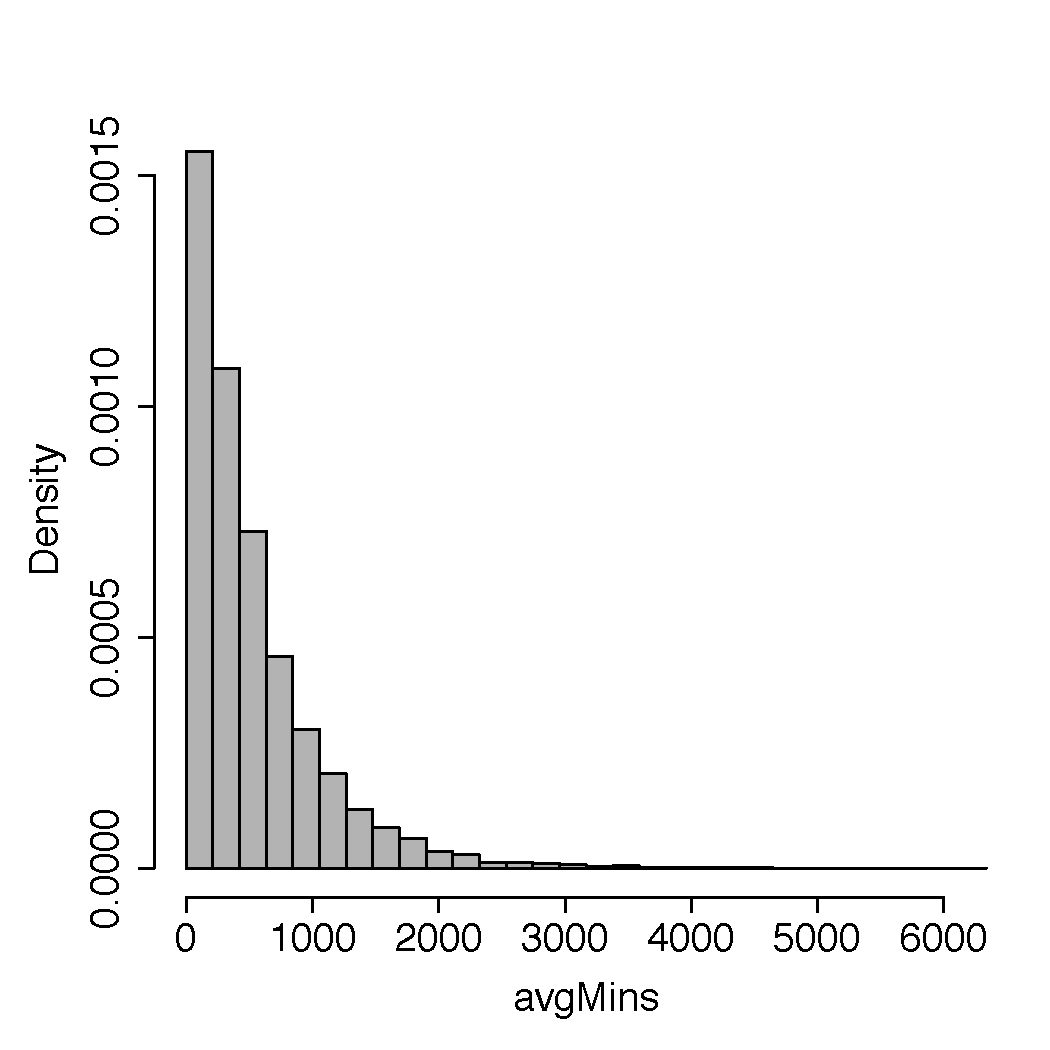
\includegraphics[width=0.24\linewidth]{./images/CaseStudy1_AcmeDQ_avgMins_hist_All.pdf}}
	\subfigure[\featN{avgReceivedMins}]{\label{fig:acmeOutlierHistogram3}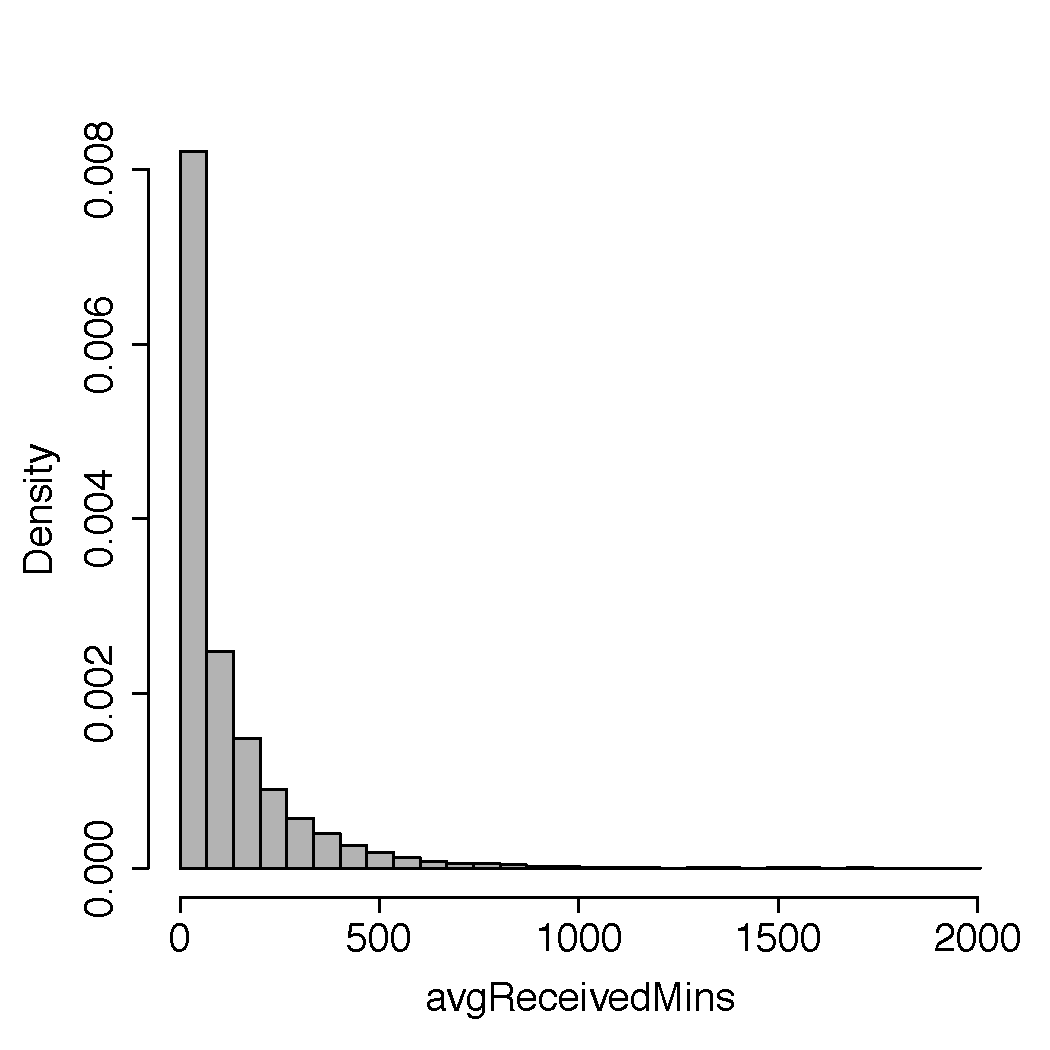
\includegraphics[width=0.24\linewidth]{./images/CaseStudy1_AcmeDQ_avgReceivedMins_hist_All.pdf}}
	\subfigure[\featN{avgOverBundleMins}]{\label{fig:acmeOutlierHistogram4}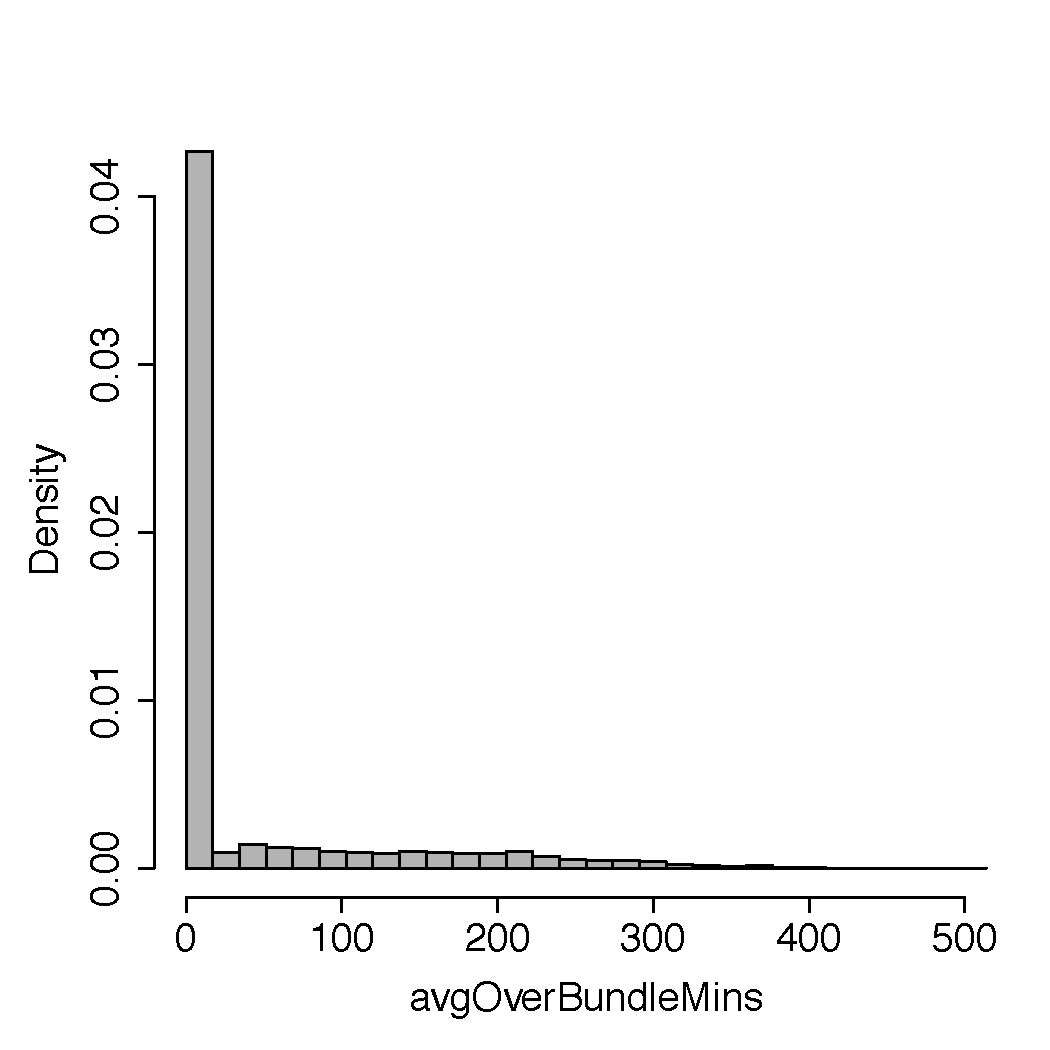
\includegraphics[width=0.24\linewidth]{./images/CaseStudy1_AcmeDQ_hacked_avgOverBundleMins_hist_All.pdf}}
\caption{(a) - (c) Histograms for the features from the AT ABT with irregular cardinality. (d) - (g) Histograms for the features from the AT ABT that are potentially suffering from outliers.}
\label{fig:acmeOutlierHistograms}
\end{figure}
\end{frame} 



 \begin{frame} 
\begin{figure}[htb]
\centering
	\subfigure[\featN{regionType}]{\label{fig:acmeABTStackedBarsRegionType}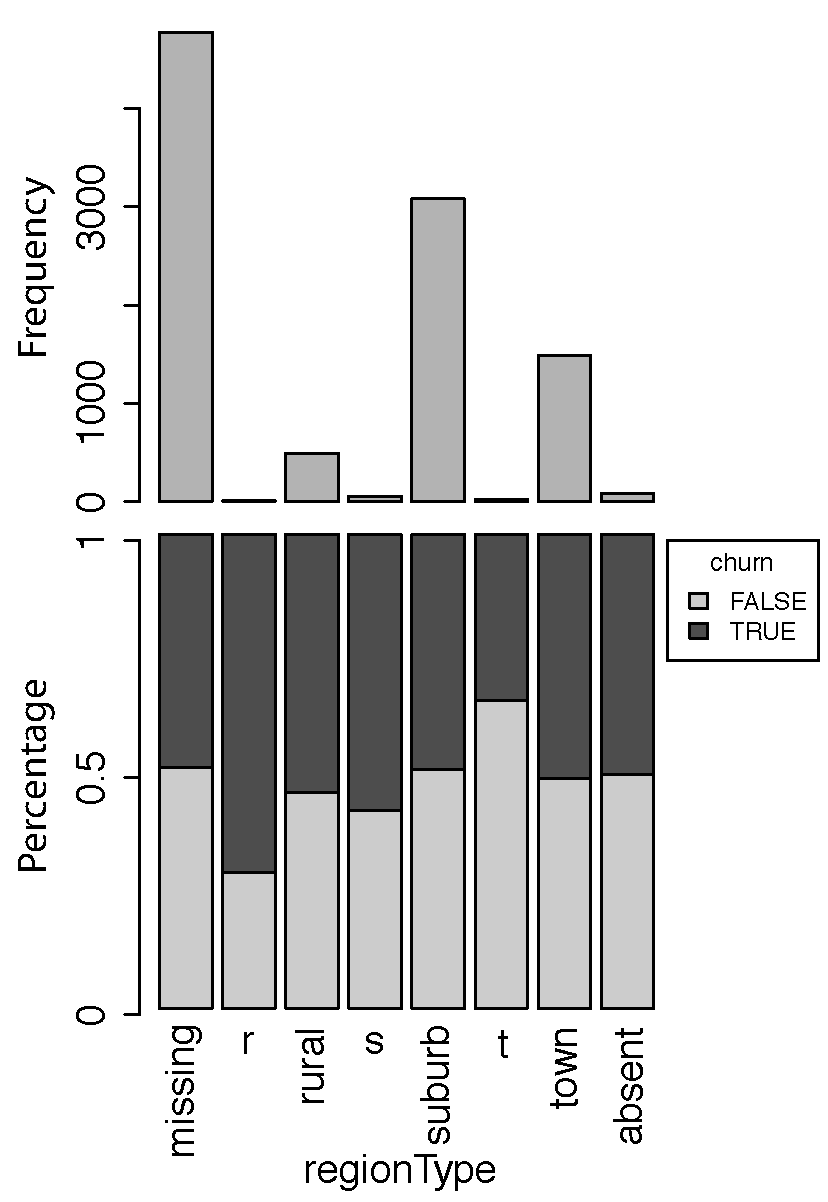
\includegraphics[width=0.32\textwidth]{./images/CaseStudy1_AcmeDQ_regionType_bar_Targets_Stacked.pdf}}
	\subfigure[\featN{avgOverBundleMins}]{\label{fig:acmeABTSmallMultHistogram1}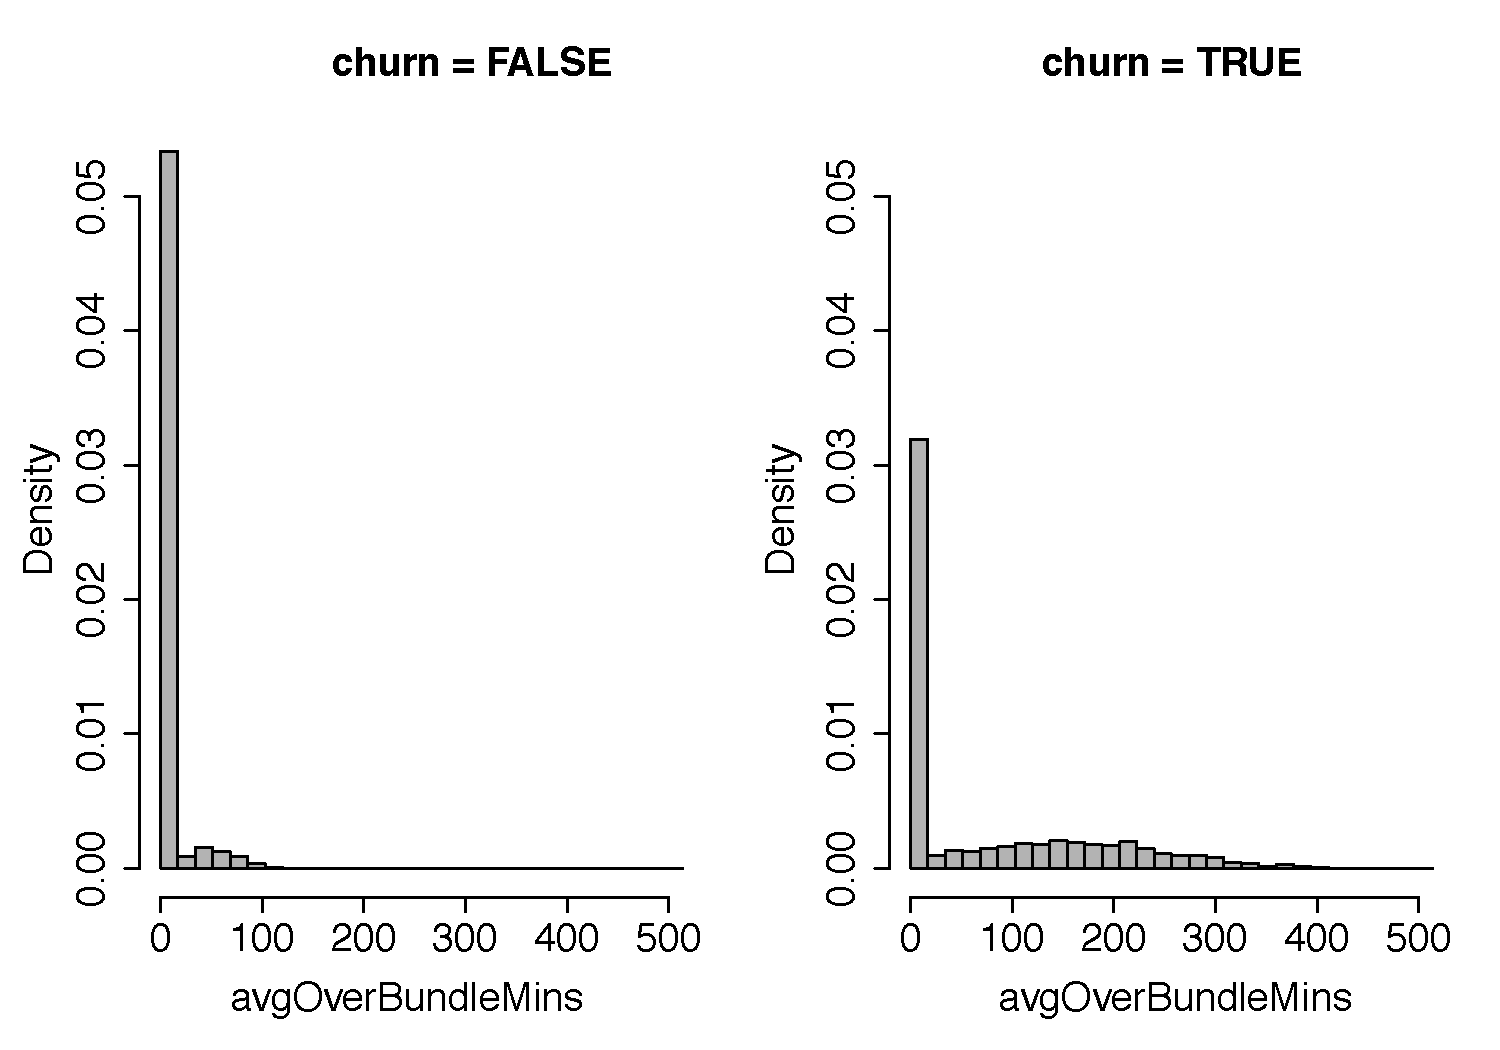
\includegraphics[width=0.6\textwidth]{./images/CaseStudy1_AcmeDQ_hacked_avgOverBundleMins_hist_Targets_mod.pdf}}
\caption{(a) a stacked bar plot for the \featN{regtionType feature}. (b) histograms for the \featN{AvgOverBundleMins} feature by target feature value.}
\label{fig:acmeDFTargetREls}
\end{figure}
\end{frame} 


\SectionSlide{Modelling}



 \begin{frame} 
\begin{figure}[!bht]
	\begin{center}
	\includegraphics[width=\textwidth]{./images/full3-wide.pdf}
	\caption{An unpruned decision tree built for the AT churn prediction problem (shown only to indicate its size and complexity). The excessive complexity and depth of the tree are evidence that over-fitting has probably occurred.}
	\label{fig:unprunedChurnTree}
	\end{center}
\end{figure}
\end{frame} 



 \begin{frame} 
\begin{figure}[!htb]
	\begin{center}
	\includegraphics[width=\textwidth]{./images/pruned-wide.pdf}
	\caption{A pruned decision tree built for the AT churn prediction problem. Grey leaf nodes indicate a churn prediction while clear leaf nodes indicate a non-churn prediction. For space reasons we only show the features tested at the top level nodes.}
	\label{fig:prunedChurnTree}
	\end{center}
\end{figure}
\end{frame} 



 \begin{frame} 
\begin{table}
\caption{The confusion matrix from the test of the AT churn prediction stratified hold-out test set using the pruned decision tree in Figure \ourRef{fig:prunedChurnTree}.}
\label{tab:telcoStratifiedConfusionMatrix}
\centering
\begin{footnotesize}
\begin{tabular}{c >{\bfseries}r @{\hspace{0.7em}} | r @{\hspace{0.4em}} r @{\hspace{0.7em}} | r @{\hspace{0.7em}}}
    & &  \multicolumn{2}{c|}{\bfseries Prediction} & \\
  & & \bfseries 	\featL{churn}		&	\bfseries \featL{non-churn} & \bfseries Recall \\
  \hline
  \multirow{2}{*}{\parbox{1.1cm}{\bfseries\raggedleft Target}}  & \textbf{\featL{churn}}		&	1,058	& 442 & 70.53\\
  &	\textbf{\featL{non-churn}}		&	152	& 1,348 & 89.86\\
\end{tabular}
\end{footnotesize}
\end{table}
\end{frame} 


\SectionSlide{Evaluation}



 \begin{frame} 
\begin{table}
\caption{The confusion matrix from the test of the AT churn prediction non-stratified hold-out test set.}
\label{tab:telcoNonStratifiedConfusionMatrix}
\centering
\begin{footnotesize}
\begin{tabular}{c >{\bfseries}r @{\hspace{0.7em}} | r @{\hspace{0.4em}} r @{\hspace{0.7em}} | r @{\hspace{0.7em}}}
    & &  \multicolumn{2}{c|}{\bfseries Prediction} & \\
  & & \bfseries 	\featL{churn}		&	\bfseries \featL{non-churn} & \bfseries Recall \\
  \hline
  \multirow{2}{*}{\parbox{1.1cm}{\bfseries\raggedleft Target}}  & \textbf{\featL{churn}}		&	1,115	 & 458 & 70.88\\
  &	\textbf{\featL{non-churn}}		&	1,439	& 12,878 & 89.95\\
\end{tabular}
\end{footnotesize}
\end{table}
\end{frame} 



 \begin{frame} 
\begin{figure}[htb]
	\begin{center}
	\subfigure[Cumulative gain]{\label{fig:treeGainLiftCharts_CumulativeGain}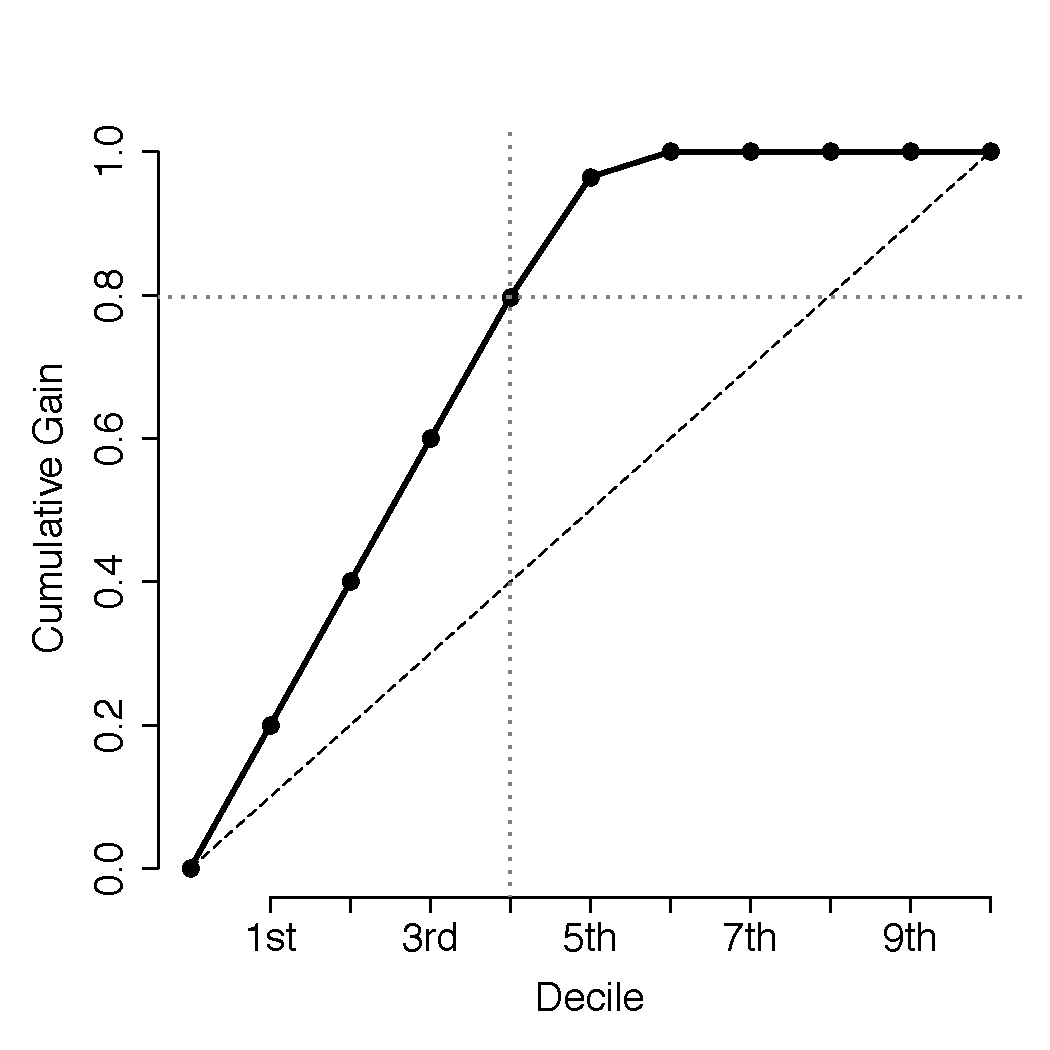
\includegraphics[width=0.32\textwidth]{./images/CaseStudy1-CumulativeGainsChart.pdf}}
	\subfigure[Lift]{\label{fig:treeGainLiftCharts_Lift}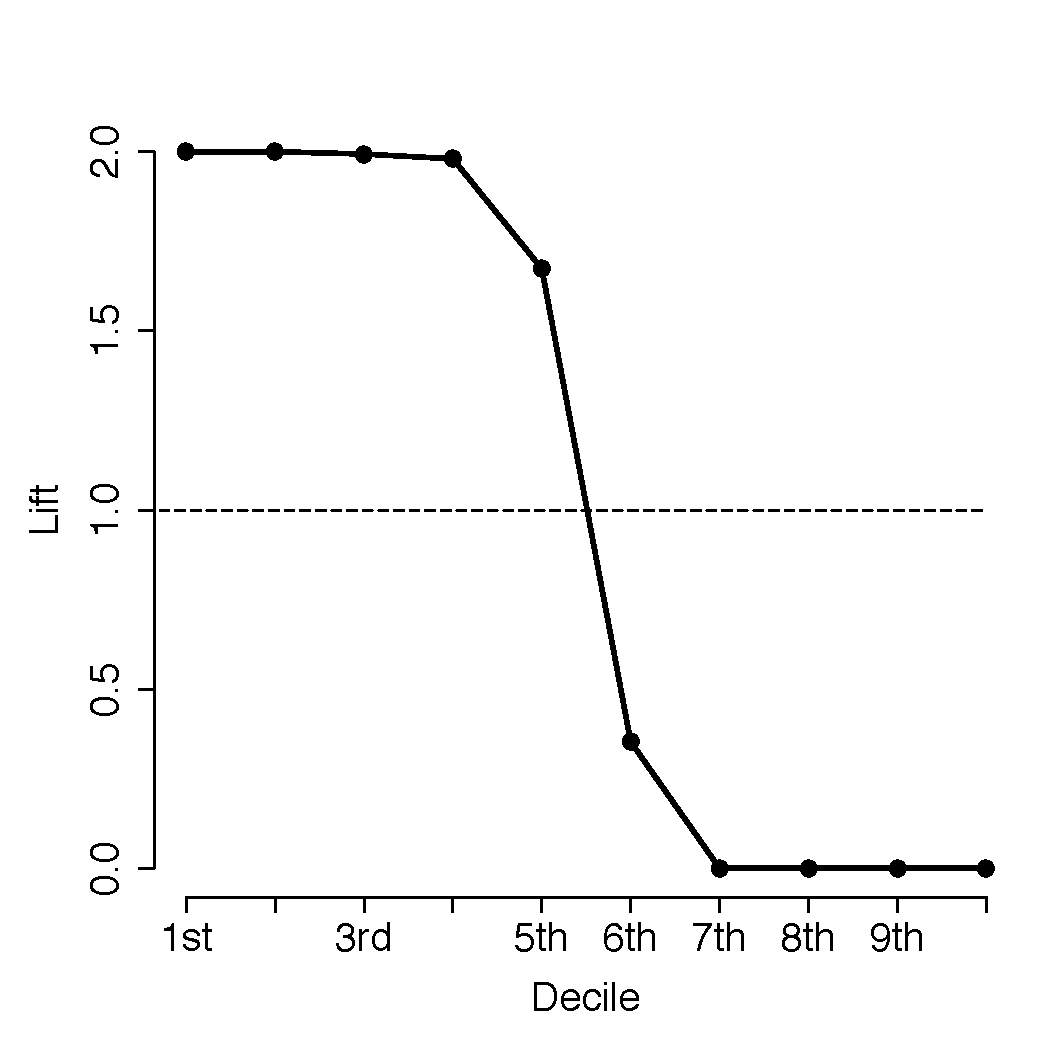
\includegraphics[width=0.32\textwidth]{./images/CaseStudy1-LiftChart.pdf}}
	\subfigure[Cumulative lift]{\label{fig:treeGainLiftCharts_CumulativeLift}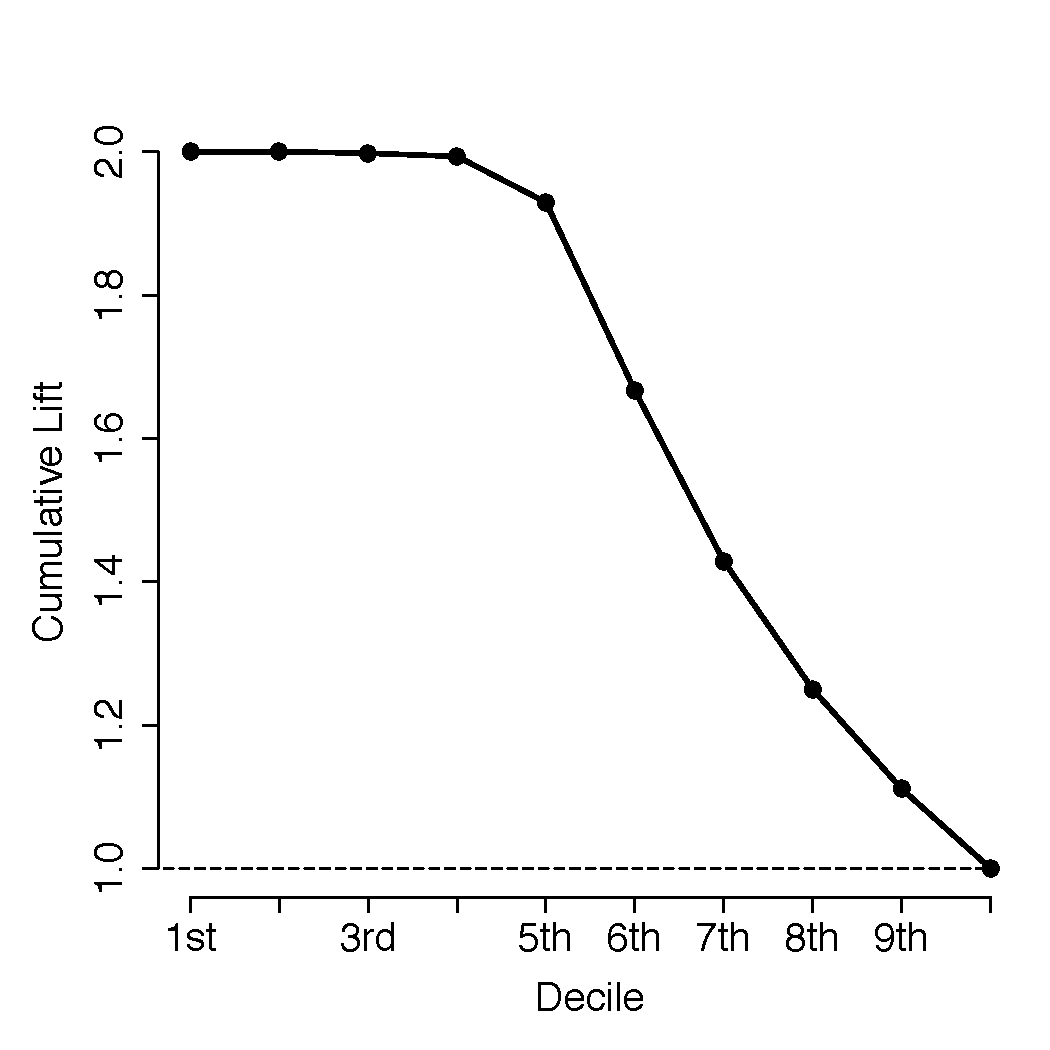
\includegraphics[width=0.32\textwidth]{./images/CaseStudy1-CumulativeLiftChart.pdf}}
	\caption{(a) cumulative gain, (b) lift and (c) cumulative lift charts for the predictions made on the large test data sample.}
	\label{fig:treeGainLiftCharts}
	\end{center}
\end{figure}
\end{frame} 



 \begin{frame} 
\begin{figure}[htb]
	\begin{center}
	\includegraphics[width=0.85\textwidth]{./images/pruned-stunted-wide.pdf}
	\caption{A pruned and stunted decision tree built for the Acme Telephonica churn prediction problem}
	\label{fig:prunedStuntedChurnTree}
	\end{center}
\end{figure}
\end{frame} 


\SectionSlide{Deployment}


 \begin{frame} 
 \begin{itemize}
\item Because AT was already using a process in which its retention team generated call lists based on collected data, deployment of the new decision tree model was reasonably straight-forward. 
\item Ross worked with the AT IT department to develop deployment-ready \keyword{extract-transform-load} (ETL) routines to generate queries for the model.
\item The last step in deployment was to put in place an \keyword{on-going model validation} plan to raise an alarm if evidence arose indicating that the deployed model had gone \keyword{stale}. 
 \end{itemize}
 \end{frame} 
 



\begin{frame}
	\tableofcontents
\end{frame}



\end{document}
